%!TEX encoding = UTF-8 Unicode

\begin{figure}
\centering
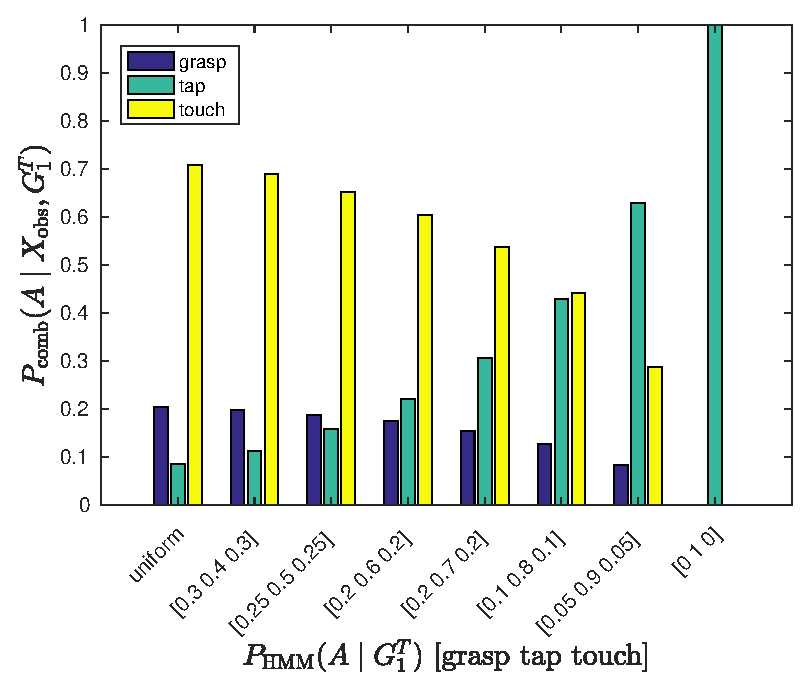
\includegraphics[width=0.9\columnwidth]{impact_of_evidence_on_Action.eps}
\caption{Predictions about the action given the evidence $\xobs =\{\text{Size}=\text{small}, \text{Shape}=\text{sphere}, \text{ObjVel}=\text{slow}\}$, combined with different probabilistic soft evidence about the action.}
\label{fig:impact_of_evidence_on_Action}
\end{figure}

\section{Experimental Results}
\label{sec:results}

In this section, we report the experimental findings obtained with our proposed model.
We present the following types of results:
\begin{itemize}
  \item inferences over affordance variables~(i.e., the entries of Table~\ref{tab:bnsymb} except the last row therein);

  \item predictions of word probabilities~(i.e., the last row of Table~\ref{tab:bnsymb});

  \item generated verbal descriptions from the word probabilities of the previous point, according to a formal grammar. The descriptions, in turn, can be interpreted to observe the emergence of certain language phenomena~(e.g., choice of most appropriate conjunction word, choice of synonym words between two consecutive sentences when they refer to the same object).
\end{itemize}

\subsection{Inference over Affordance Variables (Including Action, Synthetic Values)}

In Fig.~\ref{fig:impact_of_evidence_on_Action} we show the interaction between the \AffWords{} model and the gesture/action recognition model when they bring conflicting information.
In the scene, we observe a small ball that after the action has a low velocity (that in terms of clusters of affordance variables often corresponds to zero velocity).
Based on the evidence, the affordance model gives the highest probability $\pbn(A \given \xobs)$ to the action \emph{touch}, which usually does not result in any movement of the object.
However, in this particular simulated situation, we assume that the action performed by the human was an (unsuccessful) \emph{tap}, that is, a tap that does not result in any movement for the object.
In the simulation we show the effect of augmenting the inference with information from a gesture/action recognizer, that is, computing $\pcomb(A \given \xobs,G_1^T)$.
We analyze the effect of varying the degree of confidence of the classifier.
We start from a uniform posterior $\phmm(A \given G_1^T)$, corresponding to a poor classifier, and gradually increase the probability of the correct action until it reaches 1.
In this particular example, in order to win the belief of the affordance model, the action recognition needs to be very confident ($\phmm(A=\text{tap} \given G_1^T) > 0.81$).

\subsection{Inference over Affordance Variables (Excluding Action, Synthetic Values)}

\begin{figure*}
\centering
\subfloat[][Predictions about the object velocity of a sphere, when given different probabilistic soft evidence about the action.]
{ 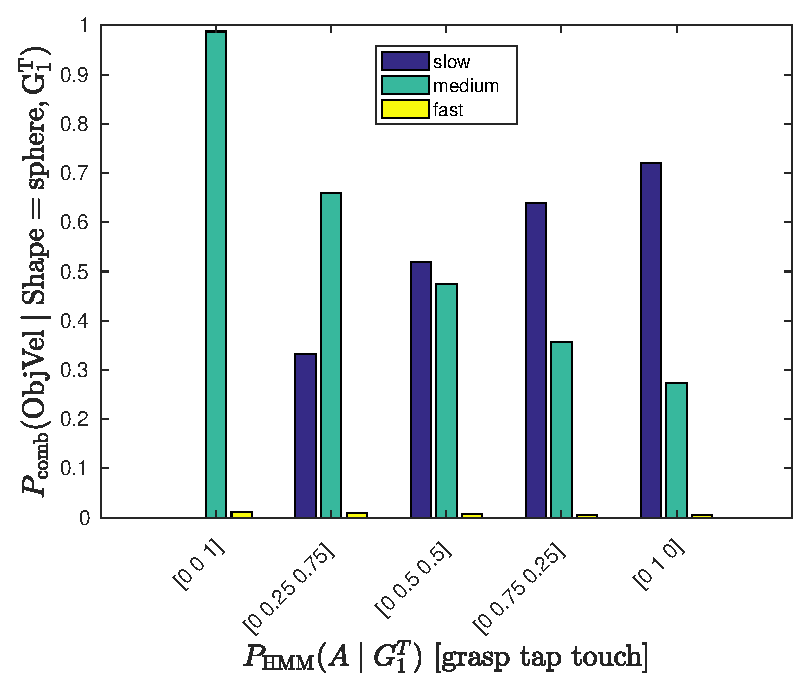
\includegraphics[width=0.45\linewidth]{impact_of_evidence_on_ObjVel_sphere.eps} \label{fig:impact_of_evidence_on_ObjVel_sphere} } \quad
%
\subfloat[][Predictions about the object velocity of a box, when given different probabilistic soft evidence about the action.]
{ 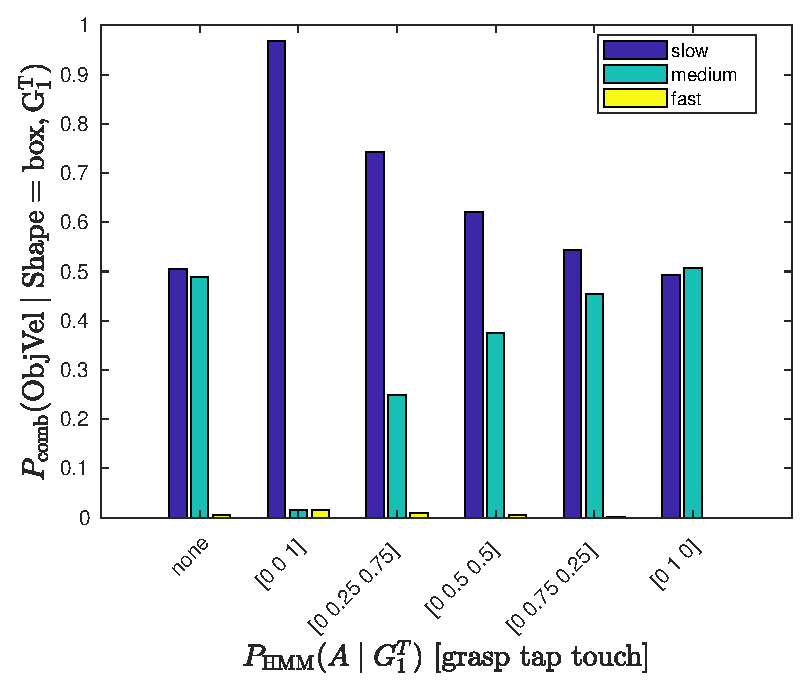
\includegraphics[width=0.45\linewidth]{impact_of_evidence_on_ObjVel_box.eps} \label{fig:impact_of_evidence_on_ObjVel_box} }
\caption{Predictions about the object velocity of different objects, when given probabilistic soft evidence about the action.}
\label{fig:impact_of_evidence_on_ObjVel}
\end{figure*}

Next, we report a result that also uses the \emph{soft evidence} over the Action node from the Gesture \acp{HMM}, but this time makes a prediction over a different node: object velocity~(which expresses an effect information).
Fig.~\ref{fig:impact_of_evidence_on_ObjVel} shows the inference in two cases: when the prior information says that the shape is spherical~(see Fig.~\ref{fig:impact_of_evidence_on_ObjVel_sphere}), and when it is cubic~(see Fig.~\ref{fig:impact_of_evidence_on_ObjVel_box}).

The first distribution to the left in both figures shows the prediction of object velocity from the \AffWords{} model alone, without any additional information.
When the shape is spherical, the model is not sure about the velocity, whereas if the shape is cubic, the model does not expect high velocities.
If we add clear evidence on the action \emph{touch} from the action recognition model, suddenly the combined model predicts slow velocities in both cases, as expected.
However, if the action recognition evidence is gradually changed from \emph{touch} to \emph{tap} the predictions of the model depend on the shape of the object.
Higher velocities are expected for spherical objects that can roll, compared to cubic objects.

\begin{figure*}
  \centering
  \subfloat[][Action perfomed on small sphere. Description: ``the robot pushed the ball and the ball moves'']{
    \resizebox{0.9\linewidth}{!}{
      \begin{tikzpicture}
        \node (lik) {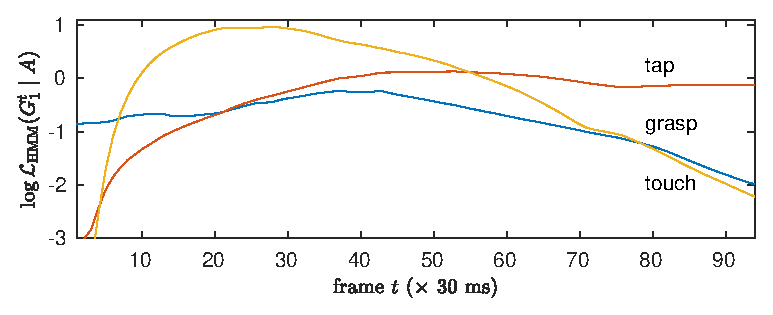
\includegraphics[width=0.6\linewidth]{evolution_of_action_posterior_sphere_log.eps}};
        \node at ([xshift=-90pt,yshift=30pt]lik.north) {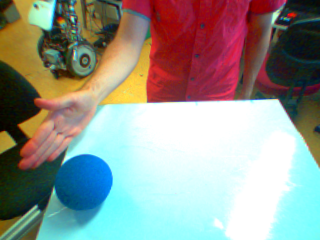
\includegraphics[width=\myWidth\linewidth]{tap-sphere-00000179}};
        \node at ([xshift=+10pt,yshift=30pt]lik.north) {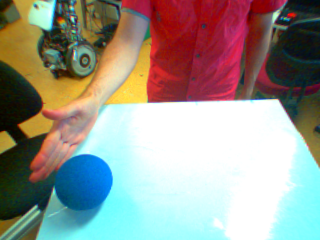
\includegraphics[width=\myWidth\linewidth]{tap-sphere-00000183}};
        \node at ([xshift=+110pt,yshift=30pt]lik.north) {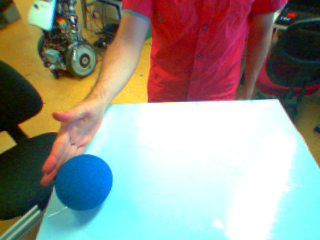
\includegraphics[width=\myWidth\linewidth]{tap-sphere-00000187}};
        \node at ([xshift=100pt,yshift=30pt]lik.east) {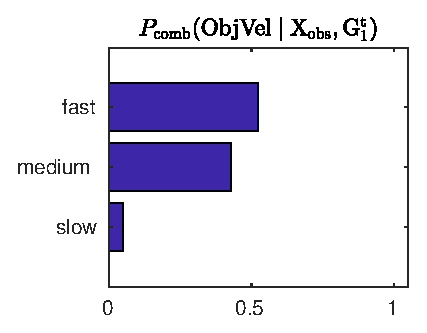
\includegraphics[width=0.35\linewidth]{evolution_of_action_posterior_sphere_effect_pred.eps}};
      \end{tikzpicture}
    } % end resizebox
    \label{fig:effect_pred_sphere}
  } % end subfloat
  
  \subfloat[][Action perfomed on big box. Description: ``the robot is pushing the big square but the box is inert'']{
    \resizebox{0.9\linewidth}{!}{
      \begin{tikzpicture}
        \node (lik) {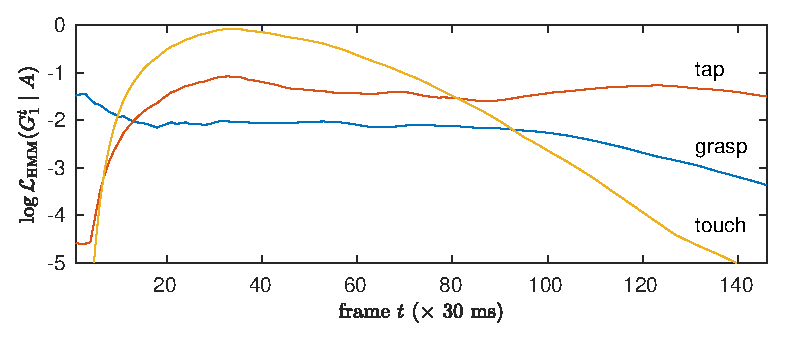
\includegraphics[width=0.6\linewidth]{evolution_of_action_posterior_box_log.eps}};
        \node at ([xshift=-90pt,yshift=30pt]lik.north) {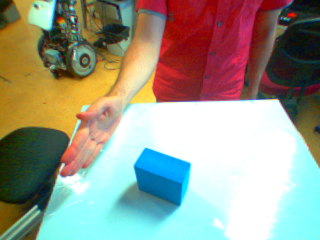
\includegraphics[width=\myWidth\linewidth]{tap-box-00000230}};
        \node at ([xshift=+10pt,yshift=30pt]lik.north) {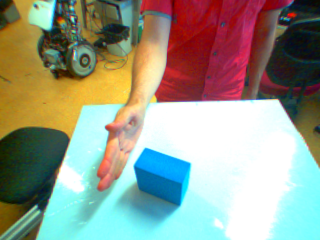
\includegraphics[width=\myWidth\linewidth]{tap-box-00000250}};
        \node at ([xshift=+110pt,yshift=30pt]lik.north) {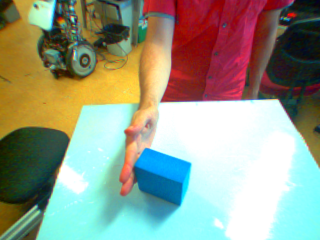
\includegraphics[width=\myWidth\linewidth]{tap-box-00000270}};
        \node at ([xshift=100pt,yshift=30pt]lik.east) {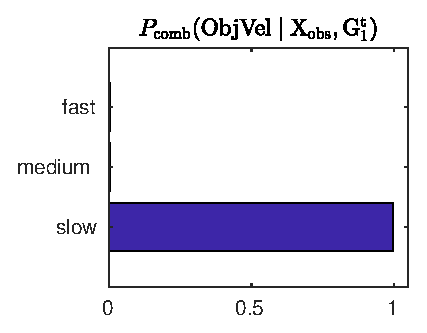
\includegraphics[width=0.35\linewidth]{evolution_of_action_posterior_box_effect_pred.eps}};
      \end{tikzpicture}
    } % end resizebox
  \label{fig:effect_pred_box}
  } % end subfloat
  \caption{Object velocity predictions before impact. The evidence from the action recognizer (left) is fed into the affodance-word model before the end of the action. The combined model predicts the effect (right) and describes it in words.}
  \label{fig:effect_pred}
\end{figure*}

\subsection{Inference and Prediction over Affordance Variables (Excluding Action, Real Values)}

Because it is based on \aclp{BN}, our model can make predictions over any set of its variables, given any other set of observed variables.
In particular, the model can do reasoning on the elements that constitute our computational concept of affordances, \textit{i.e.}, Action, Object Features, Effects in Fig.~\ref{fig:model}.
Furthermore, because the gesture/action recognition method interprets sequences of human motions, we can test this predictive ability of the complete model when we observe an incomplete action.
Fig.~\ref{fig:effect_pred} shows an example of this where we reason about the expected object velocity caused by a tap action.
Fig.~\ref{fig:effect_pred_sphere} shows the action performed on a spherical object whereas Fig.~\ref{fig:effect_pred_box} on a cubic object.
The graphs on the left side show the time evolution of the evidence $\phmm(A \given G_1^t)$ from the gesture/action recognition model.
In order to make the variations emerge more clearly, instead of the posterior, we show $\frac{1}{t}\log\mathcal{L}_\text{HMM}(G_1^t \given A)$: the log likelihood normalized by the length of the sequence.
Note how, in both cases, the correct action is recognized by the model given enough evidence, although the observation sequence is not complete.
The right side of the plot shows the prediction of the object velocity, given the incomplete observation of the action and the object properties.
Note how the model correctly predicts that the sphere will probably move but the box is unlikely do so.
Finally, the captions in the figure also show the verbal description generated by feeding the probability distribution of the words estimated by the model given the evidence into the \acl{CFG}.
%, in an anticipatory fashion, thus computing~\eqref{eq:fusion_excluding_action}.

%Note that the estimation of the human action,~$\phmm(A \given G_1^T)$, is a \emph{soft evidence}, meaning that it represents the~(time-evolving) probability distribution over the possible actions.
%Fig.~\ref{fig:effect_pred_sphere} shows the experiment when the human performs an action onto a small spherical object, whereas Fig.~\ref{fig:effect_pred_box} displays it when the object is a big box.

%      % TODO purge old pics from repo if not used
%      %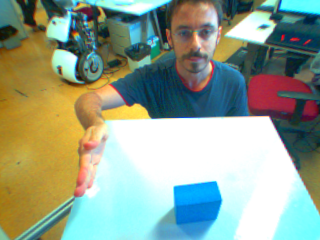
\includegraphics[width=\myWidth\linewidth]{tap-00000109}
%      %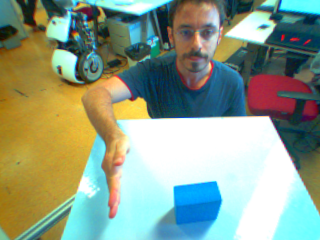
\includegraphics[width=\myWidth\linewidth]{tap-00000110}
%      %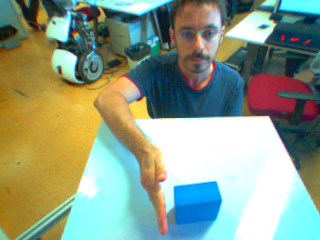
\includegraphics[width=\myWidth\linewidth]{tap-00000112}
%      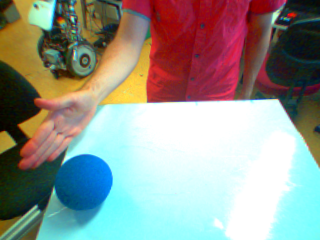
\includegraphics[width=\myWidth\linewidth]{tap-sphere-00000179}
%      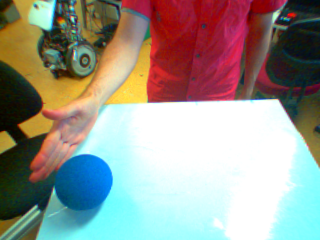
\includegraphics[width=\myWidth\linewidth]{tap-sphere-00000183}
%      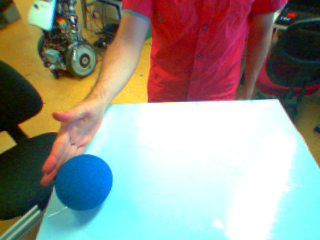
\includegraphics[width=\myWidth\linewidth]{tap-sphere-00000187}
%      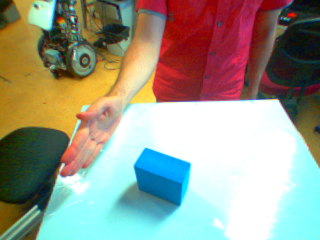
\includegraphics[width=\myWidth\linewidth]{tap-box-00000230}
%      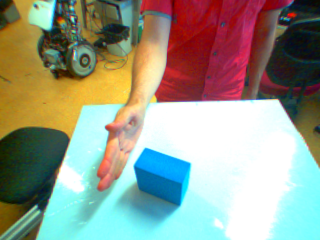
\includegraphics[width=\myWidth\linewidth]{tap-box-00000250}
%      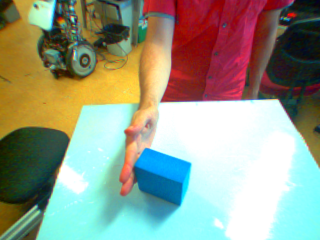
\includegraphics[width=\myWidth\linewidth]{tap-box-00000270}

%In~\ref{fig:effect_pred_sphere}, we visualize the temporal evolution of the human action likelihoods, as computed by the Gesture/Action Recognition algorithm when the human is moving the hand towards a small sphere, before the contact to the object is made.
%After about two thirds of the human movement have been completed, the model guesses correctly that it is a tap movement.
%(Before that instant, the model guesses the wrong action, in addition doing it with certainty, due to the way that the individual gestures have been modeled by continuous mixtures of Gaussian values GIAMPIERO PLEASE CHECK THIS.)
%In Fig.~\ref{fig:effect_pred_sphere}~(right), we show the prediction of the movement effect on the small sphere, before the contact is made.
%In essence, the combined model has predicted that this target object will exhibit a medium or fast velocity after the human will touch it.

%As for the experiment with the big box, Fig.~\ref{fig:effect_pred_box} shows the temporal evolution of the human action likelihoods.
%Similar considerations to the previous example apply: after about~$60$\% of the sequence has been observed, the Gesture/Action Recognition block estimates the tap correctly.
%This time, when we fuse the human action estimation to the extracted Object Features, instants below the contact occurs, we get a different result than before, show in Fig.~\ref{fig:effect_pred_box}~(right): the combined model has predicted that the object will yield a movement of type ``slow'', meaning that it will not move at all, or move slowly.
%
%These two cases have shown that, given similar human action priors~(i.e., lateral taps on a target object), the expected movement returned by the model is very different depending on the physical properties of the object.

\subsection{Prediction of Word Probabilities}

RESULT FROM GLU WITH HARD EVIDENCE

\begin{figure}
\centering
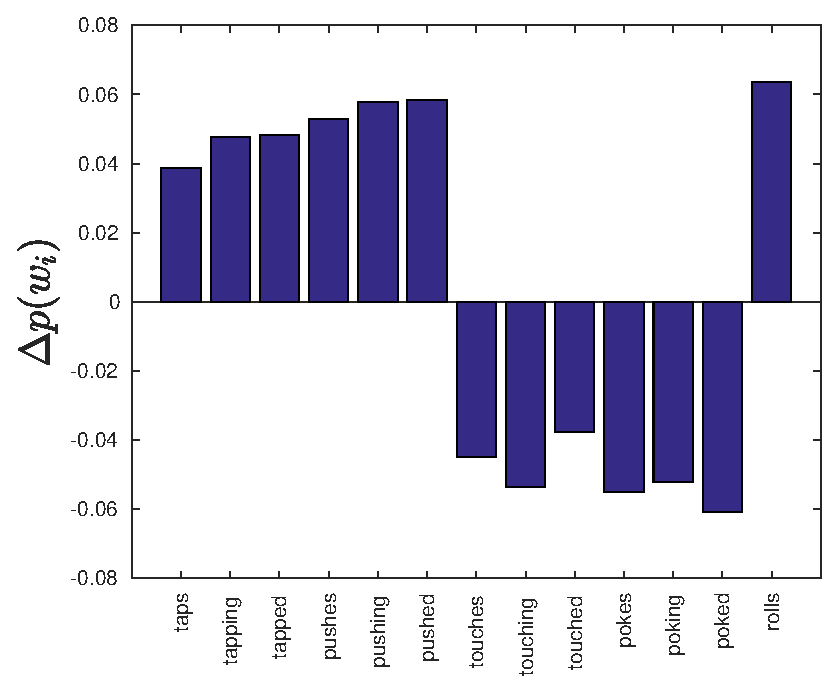
\includegraphics[width=0.9\columnwidth]{partialfig.eps}
\caption{Variation of word occurrence probabilities:
$\Delta P(w_i) = P(w_i \mid \text{InitialEvidence, Action=tap}) - P(w_i \mid \text{InitialEvidence})$, where $\text{InitialEvidence} = \{ \text{Size=big, Shape=sphere, ObjVel=fast} \}$.
This variation corresponds to the difference of word probability when we add the tap action evidence~(obtained from the Gesture \acp{HMM}) to the initial evidence about object features and effects. We have omitted words for which no significant variation was observed.}
\label{fig:probdiff}
\end{figure}

Our model permits to make predictions over the associated word descriptions in the presence or absence of an action prior.
We compare the associated \emph{verbal description} obtained by the \acl{BN} in the absence of an action prior, with the ones obtained in the presence of one.
In particular, we compare the \emph{probability of word occurrence} resulting from the following two situations:
\begin{enumerate}
\item robot prior knowledge evidence consisting of information about object features and effects only: %$\xobs^{\text{before}} = \{ \text{Size=big, Shape=sphere, ObjVel=fast} \}$;
\{Size=big, Shape=sphere, ObjVel=fast\};

\item prior evidence as in the previous situation, with the addition of the action observed from the Gestures \acp{HMM}: %$\xobs^{\text{after}} = \{ \text{Size=big, Shape=sphere, ObjVel=fast, Action=tap} \}$.
\{Size=big, Shape=sphere, ObjVel=fast, Action=tap\}.
\end{enumerate}

Fig.~\ref{fig:probdiff} shows the variation in word occurrence probabilities between the two cases, where we have omitted words for which no significant variation was observed.
We can interpret the difference in the predictions as follows: (i)~as expected, the probabilities of words related to tapping and pushing increase when a tapping action evidence from the Gestures \acp{HMM} is introduced; conversely, the probabilities of other action words~(touching and poking) decreases; (ii)~interestingly, the probability of the word \emph{rolling}~(which is an effect of an action onto an object) also increases when the tapping action evidence is entered. Even though the initial evidence of case~$1$ already included some effect information~(the velocity of the object), it is only now, when the robot perceives that the physical action was a tap, that the event rolling is associated.

\subsection{Verbal Descriptions}

%In TODO ADD REF, we have seen how our model is able to generate word probabilities after having received probabilistic observed evidence.

By generating and scoring natural language descriptions of what the robot observes~(see Sec.~\ref{sec:approach:verbal}), we can provide evidence to the model and interpret the verbal results.
Recall that with our method we do not add new words to the model, but merely generate human-readable descriptions using the same words that were present in the \AffWords{} network in the first place.
During the self-centered learning phase, the verbal descriptions of~\cite{salvi:2012:smcb} described the agent of the observed actions as either ``the~robot'', ``he'', or ``Baltazar''.
Consequently, the \AffWords{} model learned by the robot includes those words as the initial subject.

As an example, by providing the following evidence to the model:
\begin{equation} \label{eq:evidence_example}
    \xobs = \{\text{Color=yellow, Size=big, Shape=sphere, ObjVel=fast}\},
\end{equation}
we obtain
%the word probabilities of Fig.~\ref{fig:example_pw} and
the sentences reported in Table~\ref{tab:example_generated_sentences}.
The higher the score, the better.
In many of these sentences, we note that (i)~the correct action-related verb ``taps'' is generated (in the initial evidence, no action information was present, only object features and effects information were), and (ii)~the object term ``ball'' or synonyms thereof~(e.g., ``sphere'') are used coherently, both in the first part of the sentence describing the action and in the second part describing the effect.

% \begin{figure}
% \centering
% 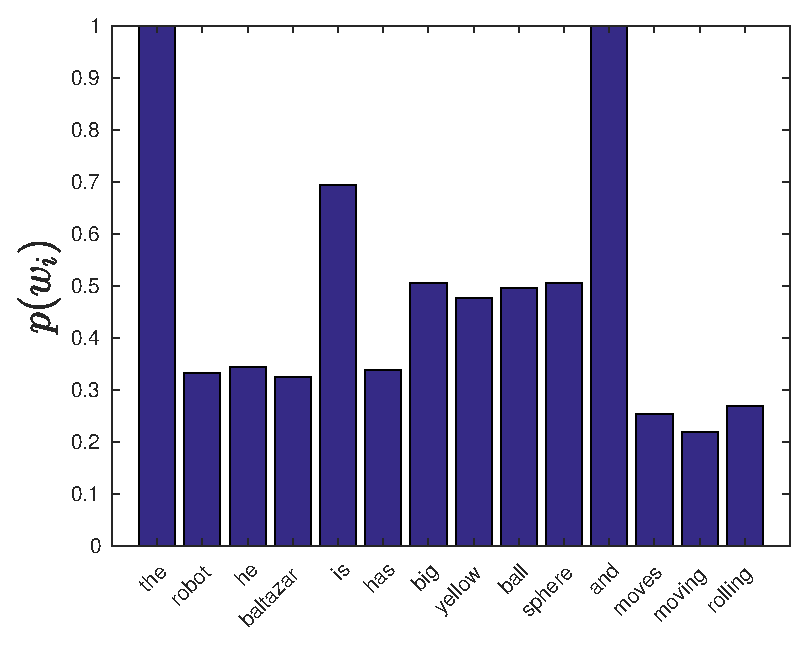
\includegraphics[width=0.9\columnwidth]{example_pw.eps}
% \caption{Word occurrence probabilities given the evidence \emph{\{Color=yellow, Size=big, Shape=sphere, ObjVel=fast\}}. We have omitted words for which no significant probability was observed.}
% \label{fig:example_pw}
% \end{figure}

\begin{table}
    \centering
    \caption{$10$-best list of sentences generated from the evidence~\eqref{eq:evidence_example}.}
    \label{tab:example_generated_sentences}
    \resizebox{\linewidth}{!}{% https://tex.stackexchange.com/a/27105/18819
    \begin{tabular}{ll}
    \toprule
    sentence & score \\
    \midrule
    ``the robot pushed the ball and the ball moves'' & $-0.54322$ \\ % not good to have push
    ``the robot tapped the sphere and the sphere moves'' & $-0.5605$ \\
    ``he is pushing the sphere and the sphere moves'' & $-0.57731$ \\
    ``the robot is tapping the yellow ball and the big yellow sphere is moving'' & $-0.57932$ \\
    ``he pushed the yellow ball and the sphere is rolling'' & $-0.58853$ \\
    ``the robot is poking the ball and the sphere is rolling'' & $-0.58998$ \\
    ``he is pushing the ball and the yellow ball moves'' & $-0.59728$ \\
    ``he pushes the sphere and the ball is moving'' & $-0.60528$ \\
    ``he is tapping the yellow ball and the ball is moving'' & $-0.60675$ \\
    ``the robot pokes the sphere and the ball is rolling'' & $-0.60694$ \\
    \bottomrule
    \end{tabular}%
    } % end resizebox
\end{table}

\subsection{Language Phenomenon: Choice of Correct Conjunction}

\newcommand{\evidenceProducingAnd}{$\xobs=$\{ Action=grasp, ObjVel=medium \}}
\newcommand{\evidenceProducingBut}{$\xobs=$\{ Action=grasp, ObjVel=slow \}}

The manipulation experiments that we consider have the following structure: an agent~(human or robot) performs a physical action onto an object with certain properties, and this object will produce a certain physical effect as a result.
For example, ``touch'' on an object yields no physical movement, but ``tap'' does~(especially if the object is spherical).
In the language description associated to an experiment, it makes sense to measure the conjunction chosen by the model given specific evidence.
In particular, it would be desirable to separate two kinds of behaviors: one in which the action and effect are coherent~(expected conjunction: ``and''), and the other one in which they are contradictory (``but'').

Fig.~\ref{tab:conjunction} shows an example of this behavior of the model.
We give the same action ``grasp'' to the model as evidence, but two values for the final object velocity.
When the object velocity is medium (Fig.~\ref{tab:conjunction:and}), the model interprets this as a successful grasp and uses the conjunction ``and'' to separate the description of the action from the description of the effect.
When the object velocity is slow (in the clustering procedure this was most often zero velocity), the model predicts this is an unsuccessful grasp and uses the conjunction ``but'', instead.

\begin{figure*}
  \centering
  \subfloat[][Evidence: \evidenceProducingAnd.]{
    \begin{tabular}[b]{c}   
    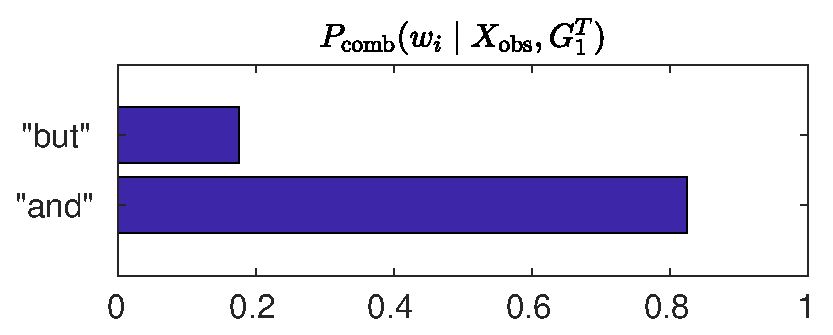
\includegraphics[width=0.4\linewidth]{p_conjunctions_and_evidence.eps}\\
    
    \resizebox{!}{0.1\linewidth}{% https://tex.stackexchange.com/a/27105/18819
      \begin{tabular}{ll}
        \toprule
        sentence & score \\
        \midrule
        ``the robot is picking the sphere \textbf{and} the sphere is moving''  & $-0.59328$ \\
        ``the robot grasps the sphere \textbf{and} the ball is moving''  & $-0.59507$ \\
        ``the robot is picking the sphere \textbf{and} the sphere is rising''  & $-0.60882$ \\
        ``the robot grasped the sphere \textbf{and} the sphere is rising''  & $-0.61842$ \\
        ``the robot picked the ball \textbf{and} the ball is rising''  & $-0.64052$ \\
        ``baltazar grasps the sphere \textbf{and} the sphere is moving''  & $-0.66182$ \\
        ``the robot has grasped the ball \textbf{and} the ball is rising''  & $-0.66398$ \\
        ``the robot picked the ball \textbf{and} the green ball is moving''  & $-0.67134$ \\
        ``baltazar grasped the sphere \textbf{and} the ball is moving''  & $-0.67283$ \\
        ``baltazar is grasping the ball \textbf{and} the sphere is rising''  & $-0.6787$ \\
        \bottomrule
      \end{tabular}%
    } % end resizebox
    \end{tabular}
    \label{tab:conjunction:and}
  } % end subfloat
  \subfloat[][Evidence: \evidenceProducingBut.]{
    \begin{tabular}[b]{c}   
    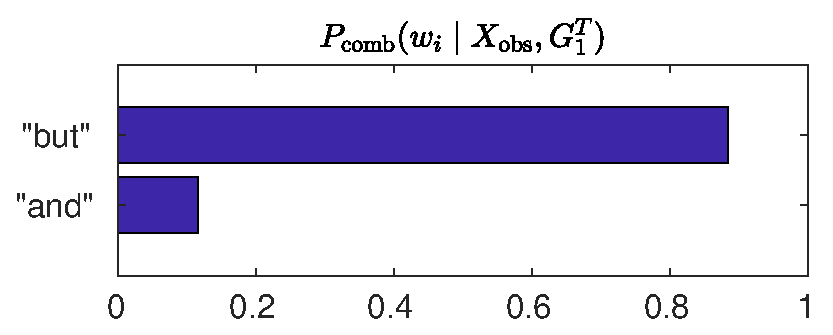
\includegraphics[width=0.4\linewidth]{p_conjunctions_but_evidence.eps}\\
    
    \resizebox{!}{0.1\linewidth}{% https://tex.stackexchange.com/a/27105/18819
      \begin{tabular}{ll}
        \toprule
        sentence & score \\
        \midrule
        ``the robot is picking the cube \textbf{but} the square is still''  & $-0.52575$ \\
        ``the robot is grasping the sphere \textbf{but} the box is inert''  & $-0.55$ \\
        ``the robot is grasping the square \textbf{but} the sphere is still''  & $-0.55388$ \\
        ``the robot grasped the square \textbf{but} the cube is inert''  & $-0.55608$ \\
        ``baltazar is grasping the square \textbf{but} the square is inert''  & $-0.5571$ \\
        ``the robot is grasping the cube \textbf{but} the ball is inert''  & $-0.56011$ \\
        ``the robot picks the box \textbf{but} the square is inert''  & $-0.56397$ \\
        ``baltazar is picking the square \textbf{but} the square is still''  & $-0.56402$ \\
        ``he is grasping the square \textbf{but} the cube is inert''  & $-0.56815$ \\
        ``the robot grasps the square \textbf{but} the sphere is inert''  & $-0.57417$ \\
        \bottomrule
      \end{tabular}%
    } % end resizebox
    \end{tabular}
    \label{tab:conjunction:but}
  } % end subfloat
    \caption{$10$-best list of sentences generated given two different sets of evidence.
    In~(a) the model interprets the object movement as indicating a succesful grasp and uses the conjunction ``and''.
    In~(b) the slow movement is interpreted as no movement at all, and, therefore, as an unsuccessful grasp: as a result, the conjunction ``but'' is used.}
    \label{tab:conjunction}
\end{figure*}

\subsection{Language Phenomenon: Verbal Description of Object Features}

\newcommand{\graspBoxGreenOne}{``the robot is grasping the box and the green box is moving''}
\newcommand{\touchBoxGreenOne}{``the robot is poking the green square and the cube is inert''}
\newcommand{\graspSphereGreenTwo}{``the robot picked the ball and the green ball is moving''}
\newcommand{\touchSphereGreenTwo}{``baltazar is poking the green sphere and the sphere is still''}

\begin{figure*}
  \centering
  \subfloat[][\graspBoxGreenOne]{
    \resizebox{0.5\linewidth}{!}{
      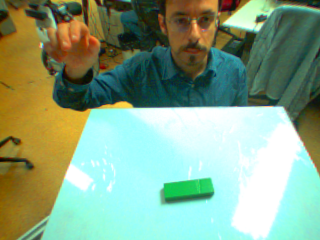
\includegraphics{graspBoxGreen1-00000007}
      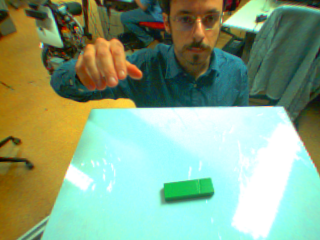
\includegraphics{graspBoxGreen1-00000008}
      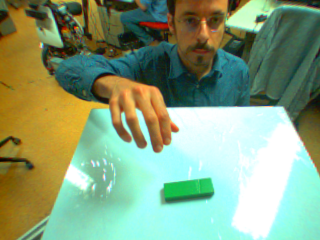
\includegraphics{graspBoxGreen1-00000009}
      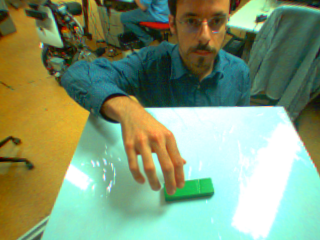
\includegraphics{graspBoxGreen1-00000010}
      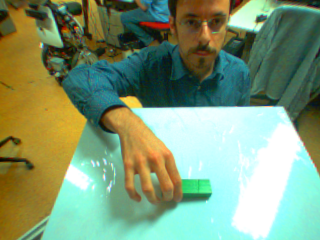
\includegraphics{graspBoxGreen1-00000013}
      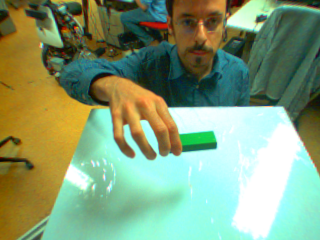
\includegraphics{graspBoxGreen1-00000016}
    } % end resizebox
  } % end subfloat
  \subfloat[][\touchBoxGreenOne]{
    \resizebox{0.5\linewidth}{!}{
      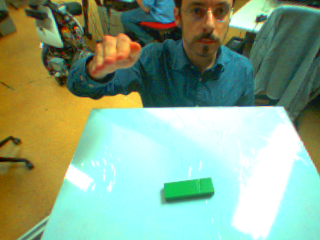
\includegraphics{touchBoxGreen1-00000008}
      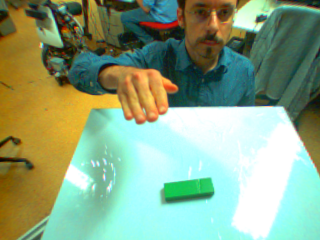
\includegraphics{touchBoxGreen1-00000009}
      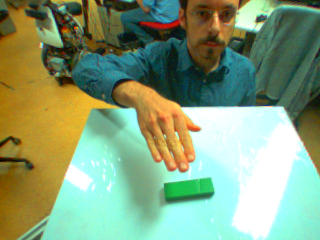
\includegraphics{touchBoxGreen1-00000010}
      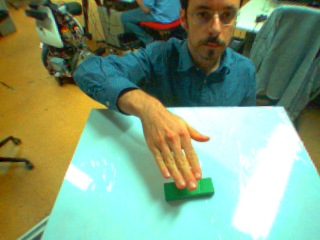
\includegraphics{touchBoxGreen1-00000011}
      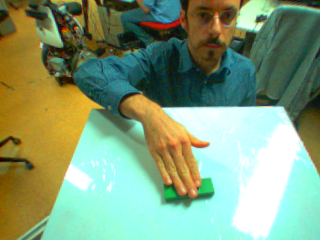
\includegraphics{touchBoxGreen1-00000013}
      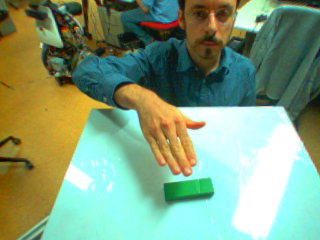
\includegraphics{touchBoxGreen1-00000015}
    } % end resizebox
  } % end subfloat

  \subfloat[][\graspSphereGreenTwo]{
    \resizebox{0.5\linewidth}{!}{
      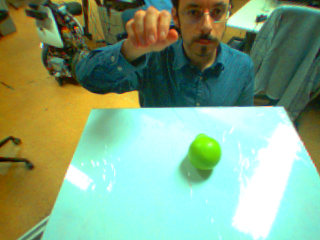
\includegraphics{graspSphereGreen2-00000007}
      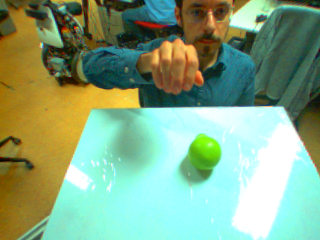
\includegraphics{graspSphereGreen2-00000008}
      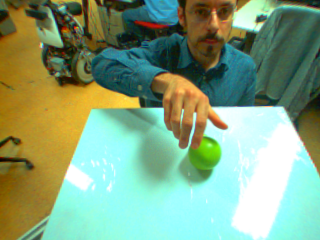
\includegraphics{graspSphereGreen2-00000009}
      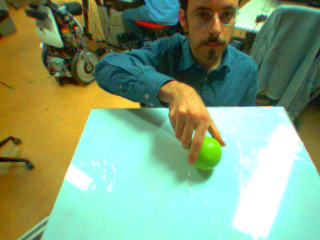
\includegraphics{graspSphereGreen2-00000011}
      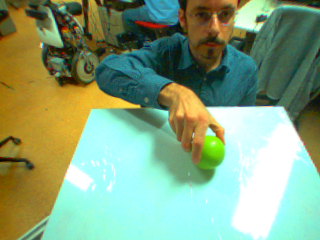
\includegraphics{graspSphereGreen2-00000013}
      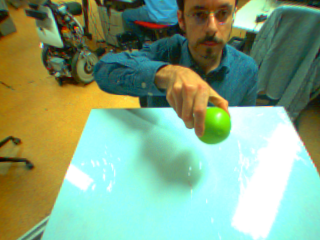
\includegraphics{graspSphereGreen2-00000015}
    } % end resizebox
  } % end subfloat
  \subfloat[][\touchSphereGreenTwo]{
    \resizebox{0.5\linewidth}{!}{
      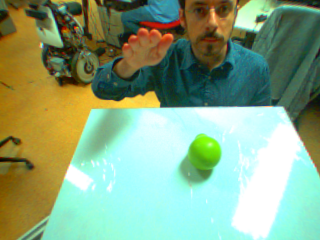
\includegraphics{touchSphereGreen2-00000006}
      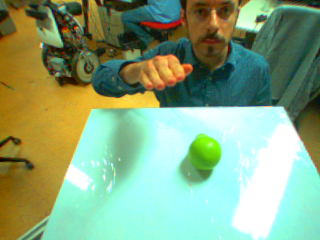
\includegraphics{touchSphereGreen2-00000007}
      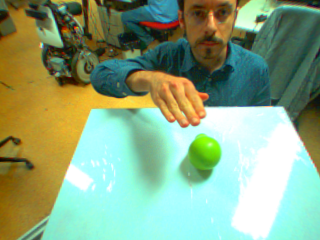
\includegraphics{touchSphereGreen2-00000008}
      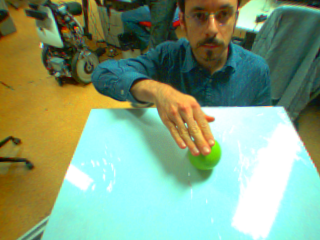
\includegraphics{touchSphereGreen2-00000010}
      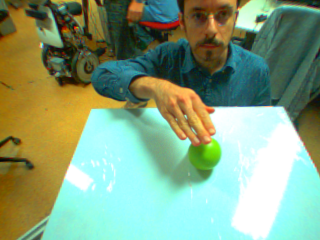
\includegraphics{touchSphereGreen2-00000011}
      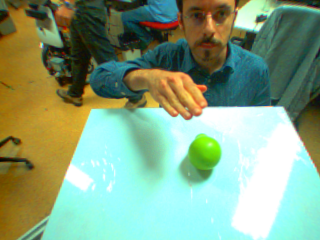
\includegraphics{touchSphereGreen2-00000012}
    } % end resizebox
  } % end subfloat

  \caption{Example of descriptions generated by the model.}
\end{figure*}


% A clarification is due: even though the conjunction ``and'' is still the most likely, the conjunction ``but'' has a comparable probability, given the observed evidence~(see Fig.~\ref{fig:conjunction_but:pw}).
% Even so, ``but'' was chosen in the highest-ranked sentence and in two more of the top-ten sentences~(see Tab.~\ref{tab:conjunction:but}).
% This result can be loosely interpreted as TODO

%\begin{figure}
%\centering
%\includegraphics[width=0.9\columnwidth]{p_conjunctions.eps}
%\caption{Word occurrence probabilities of the conjunctions ``and'' and ``but'' obtained when entering a consistent \actioneffect{} evidence vs when entering an inconsistent \actioneffect{} evidence. See Fig.~\ref{tab:conjunction} for details.}
%\label{fig:p_conjunctions}
%\end{figure}

%\subsection{Solving Ambiguities with the Combined Model}
%
%MOVE THIS RESULT EARLIER? (requires explanation of word probabilities, if we decide to include Fig.~\ref{fig:after_softevidence:pw})


%Fig.~\ref{fig:update_from_softevidence} shows the result of predictions over nodes given some initial evidence, before and after incorporating further soft evidence
%
%\begin{figure*}
%    \centering
%    \subfloat[][Prediction of the model given the initial (hard) evidence. The prediction is ambiguous.]
%    { \includegraphics[width=0.45\linewidth]{before_softevidence_prediction.eps} \label{fig:before_softevidence:pred} } \quad
%    %
%    \subfloat[][Updated prediction of the model after having incorporated the Action soft evidence (grasp tap touch)=(0.8 0.1 0.1) TODO IMPROVE NOTATION. The prediction is now unambiguous.]
%    { \includegraphics[width=0.45\linewidth]{after_softevidence_prediction.eps} \label{fig:after_softevidence:pred} }
%    \caption{Predictions about the action and hand velocity on a box object, before and after incorporating Action soft evidence from Gesture \acp{HMM}.}
%    \label{fig:update_from_softevidence}
%\end{figure*}
%
%word probabilities: Fig.~\ref{fig:after_softevidence:pw} (in this case they are identical before and after incorporating the soft evidence) REMOVE THIS?

%\begin{figure}
%\centering
%\includegraphics[width=0.9\columnwidth]{after_softevidence_pw.eps}
%\caption{Word occurrence probabilities given the evidence \{Shape=box, ObjVel=fast\}. We have omitted words for which no significant probability was observed.}
%\label{fig:after_softevidence:pw}
%\end{figure}
